% =====================================================================
%  COS212 DFS Tutor -- Software Requirements and Architecture Document
%  COS750 Educational Software Development, University of Pretoria
%  Compiles with pdfLaTeX, XeLaTeX, LuaLaTeX or Tectonic (Overleaf: pdfLaTeX)
% =====================================================================
\documentclass[11pt,a4paper]{article}

\usepackage{iftex}
\ifPDFTeX
  \usepackage[T1]{fontenc}
  \usepackage[utf8]{inputenc}
  \usepackage{lmodern}
  \usepackage[scaled=0.92]{helvet}
\else
  \usepackage{fontspec}
  \setsansfont{texgyreheros}[
    Extension=.otf, Scale=0.92,
    UprightFont=*-regular, BoldFont=*-bold,
    ItalicFont=*-italic, BoldItalicFont=*-bolditalic]
\fi

\usepackage[margin=2.3cm]{geometry}
\usepackage{microtype}
\usepackage{xcolor}
\usepackage{graphicx}
\usepackage{booktabs}
\usepackage{tabularx}
\usepackage{array}
\usepackage{longtable}
\usepackage{enumitem}
\usepackage{amsmath,amssymb}
\usepackage{float}
\usepackage{caption}
\usepackage{listings}
\usepackage{tikz}
\usetikzlibrary{arrows.meta,positioning,calc,fit,shapes.geometric,shapes.multipart,backgrounds}
\usepackage[hidelinks]{hyperref}

\setlength{\parskip}{0.45em}
\setlength{\parindent}{0pt}
\setlength{\emergencystretch}{2.5em}
\setlist{itemsep=0.15em, topsep=0.3em}
\captionsetup{font=small, labelfont=bf}
\renewcommand{\arraystretch}{1.25}
\newcolumntype{L}{>{\raggedright\arraybackslash}X}

% ---------------------------------------------------------------------
%  draw.io default palette
% ---------------------------------------------------------------------
\definecolor{dioBlueFill}{HTML}{DAE8FC}   \definecolor{dioBlueLine}{HTML}{6C8EBF}
\definecolor{dioGreenFill}{HTML}{D5E8D4}  \definecolor{dioGreenLine}{HTML}{82B366}
\definecolor{dioYellowFill}{HTML}{FFF2CC} \definecolor{dioYellowLine}{HTML}{D6B656}
\definecolor{dioOrangeFill}{HTML}{FFE6CC} \definecolor{dioOrangeLine}{HTML}{D79B00}
\definecolor{dioRedFill}{HTML}{F8CECC}    \definecolor{dioRedLine}{HTML}{B85450}
\definecolor{dioPurpleFill}{HTML}{E1D5E7} \definecolor{dioPurpleLine}{HTML}{9673A6}
\definecolor{dioGreyFill}{HTML}{F5F5F5}   \definecolor{dioGreyLine}{HTML}{666666}
\definecolor{edge}{HTML}{333333}

\tikzset{
  dio/.style={font=\sffamily\small, line width=0.75pt, >={Stealth[length=2.6mm,width=2mm,inset=0.7mm]}},
  box/.style={draw=dioBlueLine, fill=dioBlueFill, rounded corners=2.5pt, align=center,
              minimum height=9mm, minimum width=28mm, inner sep=1.5mm, font=\sffamily\small},
  boxc/.style 2 args={box, draw=#1Line, fill=#1Fill, #2},
  arrow/.style={->, draw=edge, line width=0.75pt},
  dep/.style={->, draw=edge, line width=0.75pt, dashed, >={Straight Barb[length=2.4mm,width=2.4mm]}},
  ret/.style={->, draw=edge, line width=0.7pt, dashed, >={Straight Barb[length=2mm,width=2mm]}},
  lbl/.style={font=\sffamily\scriptsize, fill=white, inner sep=1pt},
  note/.style={draw=dioYellowLine, fill=dioYellowFill, align=left, font=\sffamily\scriptsize,
               inner sep=2mm},
  treenode/.style={circle, draw=dioBlueLine, fill=dioBlueFill, minimum size=9.5mm,
                   inner sep=0pt, font=\sffamily\small\bfseries, line width=0.9pt},
  badge/.style={circle, draw=dioOrangeLine, fill=dioOrangeFill, minimum size=4.6mm,
                inner sep=0pt, font=\sffamily\scriptsize\bfseries, line width=0.6pt},
  usecase/.style={ellipse, draw=dioBlueLine, fill=dioBlueFill, minimum width=36mm,
                  minimum height=10mm, align=center, font=\sffamily\scriptsize, inner sep=0.5mm},
  umlclass/.style={rectangle split, rectangle split parts=3, draw=dioBlueLine,
                   rectangle split part fill={dioBlueFill,white,white},
                   rectangle split part align={center,left,left},
                   align=left, font=\sffamily\scriptsize, minimum width=46mm, inner sep=1.4mm},
  umlenum/.style={umlclass, rectangle split parts=2,
                  rectangle split part fill={dioPurpleFill,white}, draw=dioPurpleLine},
  stk/.style={draw=dioGreyLine, fill=dioGreyFill, minimum width=11mm, minimum height=6mm,
              font=\sffamily\small, inner sep=0pt},
  stktop/.style={stk, draw=dioOrangeLine, fill=dioOrangeFill, font=\sffamily\small\bfseries},
}

% Swimlane / container with a coloured title bar (draw.io "swimlane")
% #1 x-left, #2 y-top, #3 x-right, #4 y-bottom, #5 title, #6 colour prefix
\newcommand{\lane}[6]{%
  \draw[draw=#6Line, fill=white, line width=0.75pt] (#1,#2) rectangle (#3,#4);
  \draw[draw=#6Line, fill=#6Fill, line width=0.75pt] (#1,#2) rectangle (#3,{#2-0.62});
  \node[font=\sffamily\small\bfseries, anchor=west] at ({#1+0.25},{#2-0.31}) {#5};}

% UML stick-figure actor: #1 x, #2 y, #3 label, #4 coordinate name
\newcommand{\actor}[4]{%
  \begin{scope}[shift={(#1,#2)}, line width=0.8pt, draw=edge]
    \draw (0,0.62) circle (0.17);
    \draw (0,0.45) -- (0,-0.05);
    \draw (-0.3,0.28) -- (0.3,0.28);
    \draw (0,-0.05) -- (-0.24,-0.42);
    \draw (0,-0.05) -- (0.24,-0.42);
    \node[font=\sffamily\small] at (0,-0.68) {#3};
    \coordinate (#4) at (0,0.15);
  \end{scope}}

% UML 3-D deployment node: #1 x-left, #2 y-top, #3 x-right, #4 y-bottom, #5 title, #6 colour
\newcommand{\depnode}[6]{%
  \fill[#6Fill!70!#6Line] (#3,#2) -- ++(0.35,0.35) -- ({#3+0.35},{#4+0.35}) -- (#3,#4) -- cycle;
  \fill[#6Fill!85!#6Line] (#1,#2) -- ++(0.35,0.35) -- ({#3+0.35},{#2+0.35}) -- (#3,#2) -- cycle;
  \draw[draw=#6Line, line width=0.75pt] (#1,#2) -- ++(0.35,0.35) -- ({#3+0.35},{#2+0.35})
        -- ({#3+0.35},{#4+0.35}) -- (#3,#4);
  \draw[draw=#6Line, line width=0.75pt] (#3,#2) -- ++(0.35,0.35);
  \draw[draw=#6Line, fill=#6Fill, line width=0.75pt] (#1,#2) rectangle (#3,#4);
  \node[font=\sffamily\small, anchor=north, align=center] at ({(#1+#3)/2},{#2-0.12}) {#5};}

% ---------------------------------------------------------------------
%  Code listings
% ---------------------------------------------------------------------
\definecolor{codebg}{HTML}{F7F7F7}
\definecolor{codekw}{HTML}{1F4E94}
\definecolor{codecm}{HTML}{5A7F4B}
\definecolor{codestr}{HTML}{A0522D}
\lstdefinestyle{java}{
  language=Java, basicstyle=\ttfamily\footnotesize, keywordstyle=\color{codekw}\bfseries,
  commentstyle=\color{codecm}\itshape, stringstyle=\color{codestr},
  backgroundcolor=\color{codebg}, frame=single, rulecolor=\color{black!15},
  numbers=left, numberstyle=\tiny\color{black!45}, xleftmargin=1.6em, framexleftmargin=1.4em,
  showstringspaces=false, breaklines=true, tabsize=4, columns=fullflexible, keepspaces=true}
\lstdefinestyle{json}{
  basicstyle=\ttfamily\footnotesize, backgroundcolor=\color{codebg}, frame=single,
  rulecolor=\color{black!15}, showstringspaces=false, breaklines=true,
  stringstyle=\color{codestr}, morestring=[b]", columns=fullflexible, keepspaces=true}

\newcommand{\code}[1]{\texttt{#1}}

% =====================================================================
\begin{document}

\begin{titlepage}
  \centering
  \vspace*{2.5cm}
  {\large University of Pretoria \textperiodcentered{} Department of Computer Science\par}
  \vspace{0.3cm}
  {\large COS750 Educational Software Development\par}
  \vspace{2.2cm}
  {\Huge\bfseries COS212 DFS Tutor\par}
  \vspace{0.5cm}
  {\Large Depth-First Search on a Binary Search Tree\par}
  \vspace{0.3cm}
  {\large Software Requirements and Architecture Document (SE Document)\par}
  \vspace{2.5cm}
  \begin{tabular}{@{}ll@{}}
    \textbf{Version} & 1.1 \\
    \textbf{Date} & 28 October 2026 \\
    \textbf{Status} & Proposed baseline, awaiting team approval \\
    \textbf{Group} & \rule{6cm}{0.4pt} \\
  \end{tabular}
  \vfill
  {\small\textbf{Revision history}\par\vspace{0.2cm}}
  \begin{tabularx}{0.9\textwidth}{@{}l l L@{}}
    \toprule
    \textbf{Version} & \textbf{Date} & \textbf{Change} \\
    \midrule
    1.0 & 28 Oct 2026 & First draft. Algorithm was BST search (follow the ordering rule left or right). \\
    1.1 & 28 Oct 2026 & Algorithm changed to depth-first search (DFS). Added a plain-language
                        explanation of DFS, an educational design summary, risks and dated plan.
                        All UML diagrams redrawn. \\
    \bottomrule
  \end{tabularx}
\end{titlepage}

\tableofcontents
\newpage

% =====================================================================
\section{Introduction}
% =====================================================================

\subsection{Purpose of this document}

This is the Software Engineering (SE) document for our COS750 examination project. It records
what we are building, why, and how the pieces fit together, so that everyone in the group can
work from the same picture. The instructional design itself (learning theories, motivation,
assessment strategy, GenAI acknowledgement) is written up in full in the separate ID document, as
the examination specification requires. Section~\ref{sec:edu} gives a short summary of it here
because several software decisions only make sense once you know the teaching goal behind them.

\subsection{What we are building}

The COS212 lecturer has asked for an app that students can use \emph{before} a lecture, in the
way a tutor might sit with them for twenty minutes beforehand. We have chosen one data structure,
the \textbf{binary search tree (BST)}, and one algorithm that runs on it, \textbf{depth-first
search (DFS)}.

A student opens the app in a browser, reads a short introduction, and is shown a small tree.
They can ask the app to walk the tree depth-first, either to list every value (a traversal) or to
look for a particular value (a search). The app does not just print the answer. It plays the walk
back one step at a time: which node is being visited, what is sitting on the stack, and why the
next node is the one it is. Along the way the student is asked to predict the next move, and at
the end they take a short readiness quiz. If the quiz shows they are not comfortable yet, the app
gives them a guided review before they try again.

We are aiming for a working prototype in two weeks. That is not much time, so the plan keeps the
technology familiar to the whole group and puts the effort where it matters for learning: the
step-by-step visualisation and the feedback.

\subsection{The problem we are solving}

Students can usually recite ``DFS goes deep first'', but in our experience (and in the
literature on algorithm visualisation) they struggle when asked to \emph{apply} it. The common
difficulties are:

\begin{itemize}
  \item \textbf{Confusing depth-first with level-by-level.} After visiting the root they jump
        to its other child, which is breadth-first behaviour.
  \item \textbf{Not seeing the stack.} DFS relies on remembering where to come back to. When
        this is hidden inside recursion, the ``backtracking'' looks like magic.
  \item \textbf{Mixing up pre-, in- and post-order.} All three are depth-first. They visit the
        nodes in the same walk and differ only in \emph{when} a node is recorded.
  \item \textbf{Assuming DFS uses the BST ordering.} On a BST it is tempting to think the search
        will ``go left because the value is smaller''. Plain DFS does not do that. It explores
        blindly, which is exactly why it is a useful contrast to set up the lecture on BST search.
\end{itemize}

The app is designed around these four misconceptions. Each one has a matching explanation,
visual cue and quiz question.

\subsection{Choice of data structure and algorithm}

The examination specification asks for one core data structure from the CS2023 Foundational Data
Structures and Algorithms knowledge unit (excluding one-dimensional arrays and linked lists) and
one core algorithm that can be applied to it \cite{cs2023}. Binary search trees are listed among
the foundational data structures, and depth- and breadth-first traversals are listed among the
core graph and tree algorithms. A BST is a good host for DFS for three reasons:

\begin{enumerate}
  \item A binary tree is the simplest structure on which DFS has real choices to make (left or
        right, go deeper or back up), so the algorithm is visible without the noise of a general
        graph (no cycles, no visited set needed).
  \item An in-order DFS of a BST produces the values in sorted order. This is a satisfying
        ``aha'' moment that links the algorithm back to the data structure.
  \item Because DFS ignores the ordering, students can see for themselves that it checks more
        nodes than necessary. That question (``could we do better?'') is a natural hand-over to
        the lecture.
\end{enumerate}

\subsection{Project objectives}

When the prototype is finished, a student should be able to use it to:

\begin{enumerate}
  \item Learn what a binary search tree is, assuming no prior knowledge.
  \item Understand the ordering rule (smaller values left, larger values right).
  \item See a tree drawn clearly on screen and add values to it.
  \item Run a depth-first traversal in pre-order, in-order or post-order and follow it step by step.
  \item Run a depth-first search for a value and see whether it was found and how many nodes
        were visited.
  \item See the stack change at every step, so that backtracking makes sense.
  \item Test their understanding with a short quiz and get feedback that explains mistakes.
  \item Receive extra scaffolding (a guided review) when the quiz shows they need it.
\end{enumerate}

\subsection{Scope of the two-week prototype}

\begin{tabularx}{\textwidth}{@{}L L@{}}
  \toprule
  \textbf{In scope} & \textbf{Out of scope (first version)} \\
  \midrule
  Short introduction to trees, BSTs and DFS & User accounts and authentication \\
  A predefined example tree & Database and saved progress \\
  Inserting integers into the tree & Lecturer dashboard and analytics \\
  DFS traversal (pre-, in-, post-order) & AI-powered tutoring \\
  DFS search for a target value & Breadth-first search and other algorithms \\
  Step player with stack view and explanations & Deletion and self-balancing trees \\
  ``Predict the next node'' practice & Complex animation and gamification \\
  Readiness quiz with feedback and guided review & Mobile-first layout \\
  Reset to the example tree & \\
  \bottomrule
\end{tabularx}

These limits give us a target we can actually hit, with time left for testing, documentation and
rehearsing the demonstration.

% =====================================================================
\section{Depth-first search in plain words}
\label{sec:dfs}
% =====================================================================

This section is written for the team, but the wording is deliberately close to what students
will see in the app. If we can explain it simply here, we can explain it simply on screen.

\subsection{The idea}

Imagine you are exploring a maze. At every fork you take the left-hand passage and keep going
until you hit a dead end. Then you walk back to the most recent fork where there is still a
passage you have not tried, and you take that one. You carry on like this until you have found
what you are looking for or there is nowhere left to go.

That is depth-first search. ``Depth-first'' simply means: \emph{go as deep as you can down one
path before trying another}. Walking back to the last unexplored fork is called
\textbf{backtracking}.

In a tree, the forks are the nodes and the passages are the left and right children. A leaf is
a dead end.

\subsection{How DFS remembers where to go back to: the stack}

To backtrack, you need to remember the forks you have not finished with. DFS keeps these in a
\textbf{stack}, which works like a pile of plates: you can only add a plate to the top, and you can
only take the top plate off. The last thing you put on is the first thing you take off
(last in, first out).

The DFS search used in the app follows four simple steps:

\begin{enumerate}
  \item Put the root on the stack.
  \item Take the top node off the stack and \emph{visit} it (compare it with the target).
  \item If it is the target, stop: found. Otherwise put its right child on the stack, then its
        left child (skip any that are empty). Pushing right first means the left child ends up
        on top, so left is explored first.
  \item If the stack is empty, stop: the value is not in the tree. Otherwise go back to step 2.
\end{enumerate}

\subsection{A worked example}

Figure~\ref{fig:tree} shows the example tree the app opens with. The small orange numbers give the
order in which DFS visits the nodes (pre-order).

\begin{figure}[H]
\centering
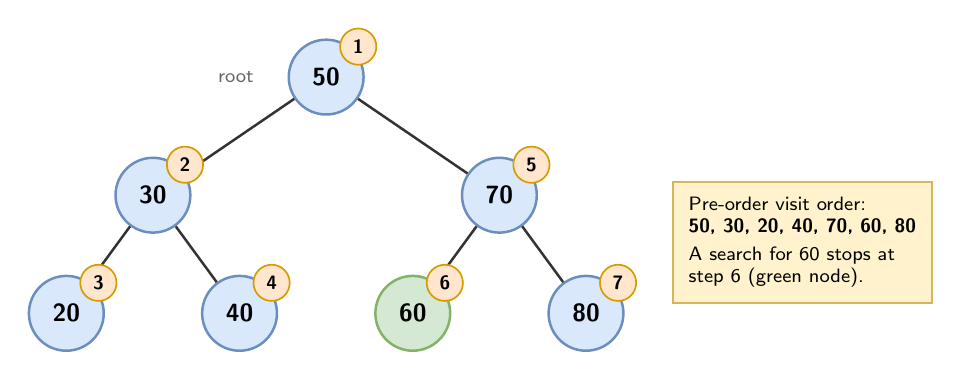
\begin{tikzpicture}[dio, level distance=15mm,
    level 1/.style={sibling distance=44mm},
    level 2/.style={sibling distance=22mm},
    every child node/.style={treenode},
    edge from parent/.style={draw=edge, line width=0.9pt}]
  \node[treenode] (n50) {50}
    child {node (n30) {30}
      child {node (n20) {20}}
      child {node (n40) {40}}}
    child {node (n70) {70}
      child {node[treenode, draw=dioGreenLine, fill=dioGreenFill] (n60) {60}}
      child {node (n80) {80}}};
  \foreach \n/\k in {n50/1, n30/2, n20/3, n40/4, n70/5, n60/6, n80/7}
    \node[badge] at ($(\n.north east)+(0.06,0.04)$) {\k};
  \node[note, anchor=west] at ($(n80.east)+(0.6,0.9)$)
    {Pre-order visit order:\\ \textbf{50, 30, 20, 40, 70, 60, 80}\\[2pt]
     A search for 60 stops at\\ step 6 (green node).};
  \node[font=\sffamily\scriptsize, text=dioGreyLine, anchor=east] at ($(n50.west)+(-0.3,0)$) {root};
\end{tikzpicture}
\caption{The example BST. Badges show the order in which a pre-order DFS visits each node.}
\label{fig:tree}
\end{figure}

Table~\ref{tab:trace} traces a search for 60. The stack is written with the top on the left.

\begin{table}[H]
\centering
\small
\begin{tabularx}{\textwidth}{@{}c c c L l@{}}
  \toprule
  \textbf{Step} & \textbf{Visit} & \textbf{Is it 60?} & \textbf{What happens} & \textbf{Stack after (top first)} \\
  \midrule
  0 & --- & --- & Start: push the root & 50 \\
  1 & 50 & no  & Push right child 70, then left child 30 & 30, 70 \\
  2 & 30 & no  & Push 40, then 20 & 20, 40, 70 \\
  3 & 20 & no  & Leaf, nothing to push. Backtrack. & 40, 70 \\
  4 & 40 & no  & Leaf, nothing to push. Backtrack. & 70 \\
  5 & 70 & no  & Push 80, then 60 & 60, 80 \\
  6 & 60 & \textbf{yes} & Found. Stop. & 80 \\
  \bottomrule
\end{tabularx}
\caption{DFS search for 60. Six nodes are visited.}
\label{tab:trace}
\end{table}

Figure~\ref{fig:stack} shows the same thing the way the app's stack panel will draw it.

\begin{figure}[H]
\centering
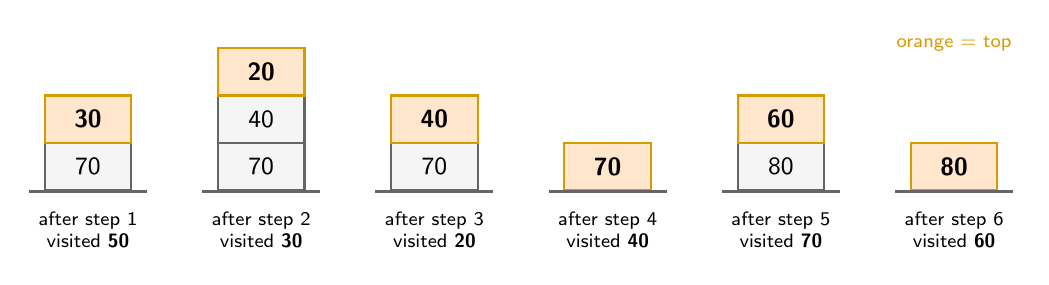
\begin{tikzpicture}[dio, x=1cm, y=1cm]
  \newcommand{\stk}[3]{\node[stk] at (#1,#2*0.6) {#3};}
  \newcommand{\stt}[3]{\node[stktop] at (#1,#2*0.6) {#3};}
  % step 1
  \stk{0}{0}{70} \stt{0}{1}{30}
  % step 2
  \stk{2.2}{0}{70} \stk{2.2}{1}{40} \stt{2.2}{2}{20}
  % step 3
  \stk{4.4}{0}{70} \stt{4.4}{1}{40}
  % step 4
  \stt{6.6}{0}{70}
  % step 5
  \stk{8.8}{0}{80} \stt{8.8}{1}{60}
  % step 6
  \stt{11}{0}{80}
  \foreach \x/\s/\v in {0/1/50, 2.2/2/30, 4.4/3/20, 6.6/4/40, 8.8/5/70, 11/6/60} {
    \draw[draw=dioGreyLine, line width=0.9pt] (\x-0.75,-0.32) -- (\x+0.75,-0.32);
    \node[font=\sffamily\scriptsize, align=center] at (\x,-0.8) {after step \s\\visited \textbf{\v}};
  }
  \node[font=\sffamily\scriptsize, text=dioOrangeLine] at (11,1.55) {orange = top};
\end{tikzpicture}
\caption{Stack contents after each step of the search for 60. The orange box is the next node to be taken off.}
\label{fig:stack}
\end{figure}

If we search for a value that is not in the tree, say 65, DFS has no way of knowing it can give
up early. It visits all seven nodes before the stack runs empty and it reports ``not found''.

\subsection{Three orders, one walk}

DFS can also be used to list every value in the tree. The walk through the tree is identical in
each case; the only difference is \emph{when} we write a node down:

\begin{table}[H]
\centering
\small
\begin{tabularx}{\textwidth}{@{}l L l@{}}
  \toprule
  \textbf{Order} & \textbf{When the node is recorded} & \textbf{Result for the example tree} \\
  \midrule
  Pre-order  & On the way down, before its children & 50, 30, 20, 40, 70, 60, 80 \\
  In-order   & Between its left and right subtree    & 20, 30, 40, 50, 60, 70, 80 \\
  Post-order & On the way back up, after its children & 20, 40, 30, 60, 80, 70, 50 \\
  \bottomrule
\end{tabularx}
\caption{The three depth-first orders on the example tree.}
\label{tab:orders}
\end{table}

Notice that the in-order result is sorted. This is not a coincidence: everything to the left of a
node is smaller and everything to the right is larger, so ``left, me, right'' produces values from
smallest to largest. The app points this out explicitly because it is the moment where the
algorithm and the data structure meet.

\subsection{What DFS does \emph{not} do, and why that matters for teaching}

DFS treats the tree as a plain tree. It does not look at the values to decide where to go. On our
example, finding 60 takes six visits, whereas a search that uses the ordering rule (``60 is bigger
than 50, go right; smaller than 70, go left'') would need only three. We show this comparison on the
summary screen as an open question for the student to bring to the lecture. It is a deliberate
cliff-hanger rather than a gap in the app.

% =====================================================================
\section{Educational design summary}
\label{sec:edu}
% =====================================================================

The full instructional design is in the ID document. This summary is here so that the
requirements in Section~\ref{sec:req} can be traced back to a teaching reason.

\subsection{Learning outcomes}

The outcomes are written against the revised Bloom's taxonomy \cite{anderson2001} so that each
quiz question can be tied to a level.

\begin{tabularx}{\textwidth}{@{}l l L@{}}
  \toprule
  \textbf{ID} & \textbf{Bloom level} & \textbf{By the end of the session, the student can\ldots} \\
  \midrule
  LO1 & Remember   & state the BST ordering rule and name the data structure DFS uses (a stack). \\
  LO2 & Understand & explain in their own words what ``depth-first'' and ``backtracking'' mean. \\
  LO3 & Apply      & write down the pre-, in- and post-order of a small BST. \\
  LO4 & Apply      & trace a DFS search for a value, giving the stack after each step. \\
  LO5 & Analyse    & predict how many nodes DFS will visit for a given target, and explain why
                     the in-order of a BST is sorted. \\
  \bottomrule
\end{tabularx}

\subsection{Instructional design approach: Gagné's Nine Events}

We use Gagné's Nine Events of Instruction \cite{gagne2005} to sequence the screens. It suits a short,
self-paced pre-lecture session because it moves from attention and prior knowledge, through
guided examples, to practice, feedback and assessment, all in one sitting. ADDIE is used as the
overall project process (analyse, design, develop, implement, evaluate) and lines up with the
development plan in Section~\ref{sec:plan}.

\begin{tabularx}{\textwidth}{@{}l L L@{}}
  \toprule
  \textbf{Gagné event} & \textbf{What the app does} & \textbf{Screen / feature} \\
  \midrule
  1 Gain attention & Short maze puzzle: ``Which way would you explore first?'' & Hook screen \\
  2 Inform of objectives & Three plain-language goals for the session & Goals card \\
  3 Recall prior learning & Two quick questions on trees and stacks; links to a refresher if needed & Warm-up check \\
  4 Present the content & Plain-language DFS explanation with the maze analogy & Concept screens \\
  5 Provide guidance & Worked example played step by step with narration & Step player \\
  6 Elicit performance & Student predicts the next node before it is revealed & Predict mode \\
  7 Provide feedback & Immediate, specific feedback on every prediction and answer & Feedback panel \\
  8 Assess performance & Six-question readiness quiz & Quiz \\
  9 Enhance retention and transfer & Summary, ``try your own tree'', questions for the lecture & Summary screen \\
  \bottomrule
\end{tabularx}

Figure~\ref{fig:journey} shows how a student moves through these screens, including the
remediation loop.

\begin{figure}[tbp]
\centering
\resizebox{\linewidth}{!}{%
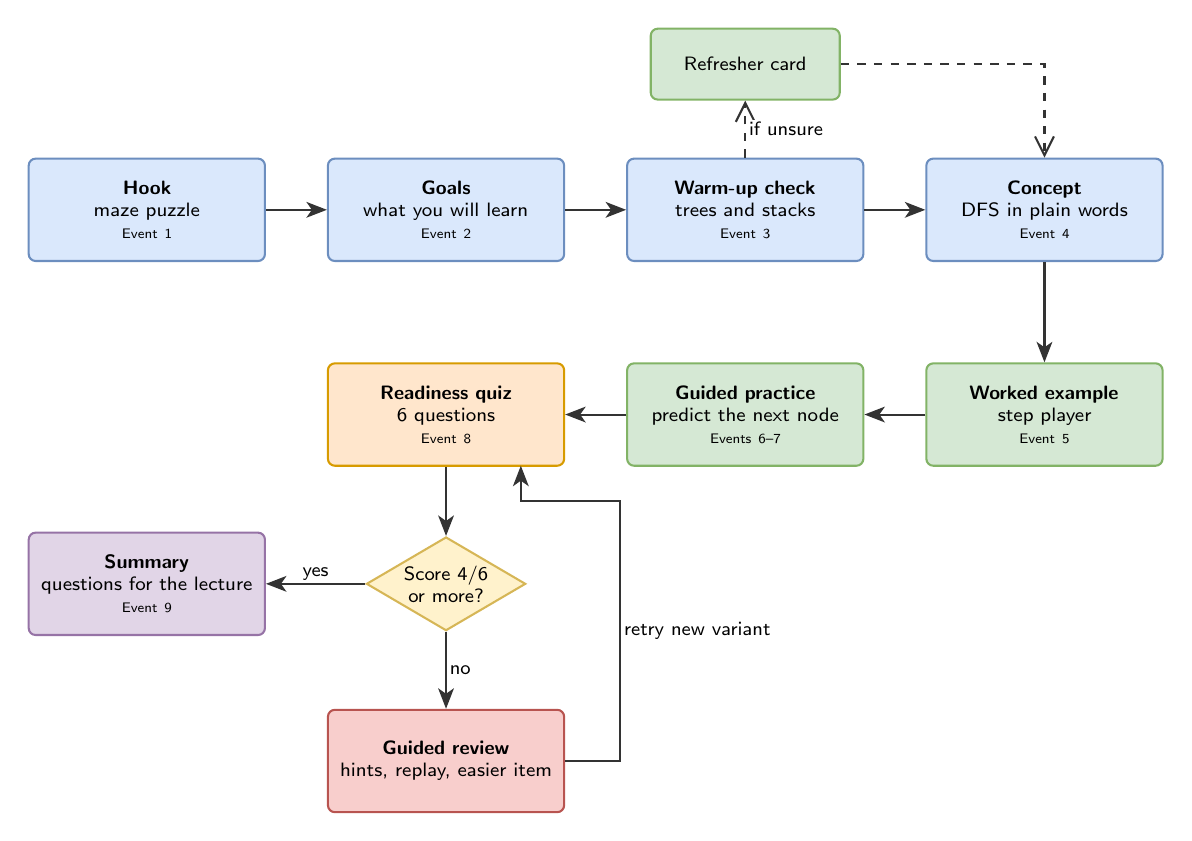
\begin{tikzpicture}[dio, node distance=7mm]
  \tikzset{jb/.style={boxc={#1}{minimum width=30mm, minimum height=13mm, text width=27mm,
                        font=\sffamily\scriptsize}}}
  \node[jb=dioBlue]  (a) at (0,0)     {\textbf{Hook}\\ maze puzzle\\ {\tiny Event 1}};
  \node[jb=dioBlue]  (b) at (3.8,0)   {\textbf{Goals}\\ what you will learn\\ {\tiny Event 2}};
  \node[jb=dioBlue]  (c) at (7.6,0)   {\textbf{Warm-up check}\\ trees and stacks\\ {\tiny Event 3}};
  \node[jb=dioBlue]  (d) at (11.4,0)  {\textbf{Concept}\\ DFS in plain words\\ {\tiny Event 4}};
  \node[jb=dioGreen] (e) at (11.4,-2.6) {\textbf{Worked example}\\ step player\\ {\tiny Event 5}};
  \node[jb=dioGreen] (f) at (7.6,-2.6)  {\textbf{Guided practice}\\ predict the next node\\ {\tiny Events 6--7}};
  \node[jb=dioOrange] (g) at (3.8,-2.6) {\textbf{Readiness quiz}\\ 6 questions\\ {\tiny Event 8}};
  \node[diamond, aspect=1.7, draw=dioYellowLine, fill=dioYellowFill, font=\sffamily\scriptsize,
        align=center, inner sep=0.3mm] (h) at (3.8,-4.75) {Score 4/6\\ or more?};
  \node[jb=dioPurple] (i) at (0,-4.75)  {\textbf{Summary}\\ questions for the lecture\\ {\tiny Event 9}};
  \node[jb=dioRed]    (j) at (3.8,-7.0) {\textbf{Guided review}\\ hints, replay, easier item};
  \node[boxc={dioGreen}{minimum width=24mm, minimum height=9mm, font=\sffamily\scriptsize}]
        (r) at (7.6,1.85) {Refresher card};
  \draw[arrow] (a) -- (b);
  \draw[arrow] (b) -- (c);
  \draw[arrow] (c) -- (d);
  \draw[arrow] (d) -- (e);
  \draw[arrow] (e) -- (f);
  \draw[arrow] (f) -- (g);
  \draw[arrow] (g) -- (h);
  \draw[arrow] (h) -- node[lbl, above] {yes} (i);
  \draw[arrow] (h) -- node[lbl, right] {no} (j);
  \draw[arrow] (j.east) -- ++(0.7,0) |- node[lbl, pos=0.25, right] {retry new variant} (4.75,-3.7) -- (4.75,-3.25);
  \draw[dep] (c.north) -- node[lbl, right] {if unsure} (r.south);
  \draw[dep] (r.east) -| (d.north);
\end{tikzpicture}}
\caption{Student learning journey. Blue: instruction; green: guided practice; orange: assessment; red: remediation; purple: consolidation.}
\label{fig:journey}
\end{figure}

\subsection{Learning theories in practice}

\begin{description}[style=nextline, leftmargin=1.2em]
  \item[Cognitive load theory \cite{sweller1988}.] DFS has a lot going on at once: the tree, the
        current node, the stack and the order. We reduce load by \emph{segmenting} (one step per
        click), \emph{signalling} (colour for current, visited, on-stack and found nodes) and
        keeping explanation text right next to the diagram rather than in a separate panel. The
        student controls the pace; there is no auto-play that runs ahead of them.
  \item[Worked examples and fading.] The first example is fully worked. In the second the student
        predicts the next node and the app confirms. In the third they trace on their own. This
        follows the worked-example effect and its fading strategy, which is well suited to novices.
  \item[Active learning and engagement.] Research on algorithm visualisation shows that
        \emph{watching} an animation adds little; learning improves when students have to respond
        to it or change it \cite{hundhausen2002, naps2002}. ``Predict the next node'' puts students
        at the \emph{responding} level of the engagement taxonomy, and inserting their own values
        puts them at the \emph{changing} level.
  \item[Scaffolding and the zone of proximal development \cite{vygotsky1978}.] Hints are layered:
        a nudge first (``Which node is on top of the stack?''), then a stronger hint, then the
        answer with an explanation. The guided review is the app acting as the ``more
        knowledgeable other'' for students who are not ready yet.
  \item[Dual coding and multiple representations \cite{mayer2009}.] Every step is shown as a
        picture (the tree), a structure (the stack), words (the explanation) and, optionally,
        code (the highlighted line in the Java method).
\end{description}

\subsection{Catering for different learners}

The specification asks which learning styles the app caters for. We map our features onto the
VARK categories because they are familiar, but we are careful not to over-claim: there is little
evidence that matching teaching to a preferred style improves results \cite{pashler2008}. Our
approach is therefore to give \emph{every} student several representations, which helps all
learners regardless of preference.

\begin{tabularx}{\textwidth}{@{}l L@{}}
  \toprule
  \textbf{VARK category} & \textbf{How the app supports it} \\
  \midrule
  Visual      & Tree diagram, colour-coded states, animated stack panel. \\
  Aural       & Optional read-aloud of step explanations using the browser's built-in speech
                synthesis (``Could'' priority). \\
  Read/write  & Short text explanations, a glossary, the Java code view. \\
  Kinaesthetic & Stepping manually, predicting, inserting values and building their own tree. \\
  \bottomrule
\end{tabularx}

Accessibility is treated as a requirement, not an extra: node states are never shown by colour
alone (each also has an icon or outline style), all controls work from the keyboard, and text
meets WCAG AA contrast.

\subsection{Motivation (ARCS)}

We use Keller's ARCS model \cite{keller1987} to keep students engaged for the twenty minutes or so a
session takes.

\begin{tabularx}{\textwidth}{@{}l L@{}}
  \toprule
  \textbf{ARCS} & \textbf{Design choice} \\
  \midrule
  Attention    & Maze hook; predict-then-reveal creates small moments of suspense. \\
  Relevance    & Links to things students use: folder trees, undo history, and the COS212 practicals. \\
  Confidence   & Clear goals, short steps, early easy wins, and a progress bar showing where they are. \\
  Satisfaction & Immediate feedback, the ``sorted in-order'' discovery, and a summary of what they now know. \\
  \bottomrule
\end{tabularx}

\subsection{Assessment and scaffolding}

Assessment is formative. Its job is to tell the student (not the lecturer) whether they are ready
for the lecture, and to help them if they are not. Each question is tied to a learning outcome
and wrong options are built from the misconceptions listed in Section~1.3, so the feedback can say
\emph{why} an answer is wrong, not only that it is wrong.

\begin{longtable}{@{}p{0.6cm} p{5.4cm} p{1.4cm} p{7.4cm}@{}}
  \toprule
  \textbf{Q} & \textbf{Question (example tree)} & \textbf{LO} & \textbf{Feedback on the typical wrong answer} \\
  \midrule
  \endhead
  1 & Which structure does DFS use to remember where to go back to? & LO1 &
      \emph{Queue}: ``A queue serves the oldest item first, which explores level by level.
      That is breadth-first search. DFS needs the newest item first: a stack.'' \\
  2 & DFS has just visited 30. Which node is visited next? & LO2 &
      \emph{70}: ``70 is on the same level as 30. Depth-first goes \emph{down} before across, so the
      next node is 30's left child, 20.'' \\
  3 & Give the pre-order of the tree. & LO3 &
      \emph{20, 30, 40, \ldots}: ``That is in-order. In pre-order a node is written down
      \emph{before} its children, so the root 50 comes first.'' \\
  4 & The stack is [40, 70] (top first). What is popped next? & LO4 &
      \emph{70}: ``The top of the stack is on the left. The last node pushed was 40, so 40 comes off first.'' \\
  5 & How many nodes does DFS visit to find 80? & LO5 &
      \emph{3}: ``Three would be right if DFS used the ordering rule. Plain DFS explores the whole
      left subtree first, so it visits all 7 nodes.'' \\
  6 & Why is the in-order of a BST always sorted? & LO5 &
      Explanation built from ``left is smaller, right is larger''; a diagram highlights each subtree. \\
  \bottomrule
\end{longtable}

\textbf{Scaffolding rule.} A student who scores 4/6 or more goes to the summary screen. Below
that, the app opens a guided review that targets the outcomes they missed: it replays the
relevant part of the worked example, asks an easier version of the question with a hint, and
then offers a fresh variant of the quiz (different tree, same outcomes). The student can always
choose to continue to the summary; the review is offered, not forced.

\subsection{Use of generative AI}

The specification allows GenAI for content and GUI work, provided it is acknowledged. Any prompts
used to draft lesson text, quiz items or interface code, and the tool used, will be recorded in
an appendix of the ID document. All generated quiz items are checked by two group members
against the reference Java implementation before they go into the app.

% =====================================================================
\section{Technology stack}
% =====================================================================

The backend is Java, so the simplest path is a single Spring Boot application that serves both the
REST API and a plain HTML, CSS and JavaScript frontend.

\begin{tabularx}{\textwidth}{@{}l l L@{}}
  \toprule
  \textbf{Component} & \textbf{Technology} & \textbf{Purpose} \\
  \midrule
  Backend            & Java 21, Spring Boot 3          & BST and DFS logic; REST endpoints. \\
  Frontend           & HTML, CSS, JavaScript (no framework) & Lesson screens, step player, quiz. \\
  API                & REST with JSON                  & Browser to backend communication. \\
  Tree visualisation & SVG generated in JavaScript     & Draws nodes, edges and highlights. \\
  Build              & Maven                           & Dependencies, compilation, tests. \\
  Unit testing       & JUnit 5                         & Tests for insertion, DFS orders and search. \\
  Version control    & Git and GitHub                  & Issues, pull requests, code review. \\
  Deployment         & Local machine (\code{localhost:8080}) & Simple to run for the demonstration. \\
  \bottomrule
\end{tabularx}

\textbf{Recommended decision.} Put the frontend in \code{src/main/resources/static} so Spring Boot
serves it. One command (\code{mvn spring-boot:run}) then starts the whole prototype, with no
separate frontend server and no database. The browser calls the backend with relative URLs such as
\code{/api/dfs/search}, which means nothing has to change if we later host it elsewhere.

If some members already have Java 17 installed and working, Java 17 with a compatible Spring Boot
3 release is fine. Whatever we choose, we pin it in \code{pom.xml} so the build is the same on
every machine.

% =====================================================================
\section{Requirements}
\label{sec:req}
% =====================================================================

\subsection{Functional requirements}

Priorities use MoSCoW: \textbf{M}ust, \textbf{S}hould, \textbf{C}ould.

\begin{longtable}{@{}p{1.2cm} p{11.2cm} p{0.9cm} p{1.1cm}@{}}
  \toprule
  \textbf{ID} & \textbf{Requirement} & \textbf{Pri.} & \textbf{Trace} \\
  \midrule
  \endhead
  FR-01 & Show an introduction to trees, BSTs and DFS that assumes no prior knowledge. & M & LO1, LO2 \\
  FR-02 & Show the predefined example BST when the student opens the explorer. & M & LO3 \\
  FR-03 & Let the student insert an integer into the tree, following the BST rule. & M & LO1 \\
  FR-04 & Let the student choose a DFS order (pre-, in- or post-order) and run a traversal. & M & LO3 \\
  FR-05 & Let the student enter a target value and run a DFS search (pre-order). & M & LO4 \\
  FR-06 & Play the DFS back one step at a time, with next, previous and restart controls. & M & LO2, LO4 \\
  FR-07 & At each step, highlight the current node, mark visited nodes and show the stack. & M & LO4 \\
  FR-08 & At each step, show a one-sentence explanation of what happened and why. & M & LO2 \\
  FR-09 & After a search, show whether the target was found and how many nodes were visited. & M & LO5 \\
  FR-10 & Offer a ``predict the next node'' mode with immediate feedback. & M & LO4 \\
  FR-11 & Provide a readiness quiz linked to the learning outcomes. & M & all \\
  FR-12 & Give specific feedback that explains both correct and incorrect answers. & M & all \\
  FR-13 & Offer a guided review when the quiz score is below the threshold. & M & all \\
  FR-14 & Let the student reset the tree to the example. & S & --- \\
  FR-15 & Show a skewed tree (values inserted in sorted order) and how DFS behaves on it. & S & LO5 \\
  FR-16 & Show the matching line of Java code alongside each step. & S & LO2 \\
  FR-17 & Read step explanations aloud on request. & C & --- \\
  \bottomrule
\end{longtable}

\subsection{Non-functional requirements}

\begin{longtable}{@{}p{1.4cm} p{13.2cm}@{}}
  \toprule
  \textbf{ID} & \textbf{Requirement} \\
  \midrule
  \endhead
  NFR-01 & \textbf{Usability.} A first-year student can complete the session without help. Checked
           with at least three peer testers before the demo. \\
  NFR-02 & \textbf{Responsiveness.} Results appear within 300\,ms on a laptop for trees of up to 15 nodes. \\
  NFR-03 & \textbf{Correctness.} The steps shown in the browser come from the Java algorithm, never from a
           separate JavaScript re-implementation, so the two cannot disagree. \\
  NFR-04 & \textbf{Error messages.} Invalid input produces a short, friendly message that says what
           to do next. No stack traces are shown to students. \\
  NFR-05 & \textbf{Compatibility.} Works in current Chrome, Firefox, Edge and Safari on a laptop screen. \\
  NFR-06 & \textbf{Accessibility.} Keyboard operable; colour is never the only signal; WCAG AA contrast. \\
  NFR-07 & \textbf{Maintainability.} Java classes have one clear responsibility each; the BST and DFS
           classes do not depend on Spring. \\
  NFR-08 & \textbf{Testability.} BST insertion and every DFS order have automated JUnit tests. \\
  NFR-09 & \textbf{Portability.} The app runs locally from the README instructions with one command. \\
  NFR-10 & \textbf{Pacing.} The student controls every step; nothing advances without their action. \\
  \bottomrule
\end{longtable}

\subsection{Business rules}

\textbf{Tree rules}
\begin{enumerate}[label=BR-\arabic*, leftmargin=3.2em]
  \item Every node holds a whole number from 0 to 99 (two digits keep the circles readable).
  \item A value smaller than a node goes into that node's left subtree.
  \item A value larger than a node goes into that node's right subtree.
  \item Duplicate values are rejected with an explanation.
  \item A tree holds at most 15 nodes so that it fits on a laptop screen.
\end{enumerate}

\textbf{DFS rules}
\begin{enumerate}[label=BR-\arabic*, leftmargin=3.2em, start=6]
  \item Every DFS starts at the root.
  \item DFS goes as deep as possible along one branch before backtracking.
  \item The left child is always explored before the right child (matches the COS212 convention).
  \item DFS search checks each node when it is first reached (pre-order) and stops as soon as the
        target is found or the stack is empty.
  \item ``Nodes visited'' counts only real nodes, never empty (null) children. Each node is visited
        at most once.
  \item DFS does \emph{not} use the ordering of the BST to skip subtrees. This is intentional: it is
        what makes it DFS rather than BST search.
\end{enumerate}

% =====================================================================
\section{System architecture}
% =====================================================================

\subsection{Architecture decision}

We use a simple layered architecture inside one Spring Boot application:

\begin{itemize}
  \item The \textbf{browser} handles everything the student sees: lesson screens, the SVG tree, the
        step player and the quiz.
  \item A \textbf{controller} layer turns HTTP requests into method calls and results into JSON.
  \item A \textbf{service} layer holds the current tree and coordinates the work.
  \item A \textbf{domain} layer contains the BST and the DFS algorithm as plain Java, with no
        Spring code, so they can be unit-tested directly.
\end{itemize}

The algorithm is kept separate from the data structure (\code{DepthFirstSearch} operates on a
\code{BinarySearchTree} rather than being a method inside it). This mirrors how we want students to
think: the tree is one idea, the walk over it is another.

There is no database. The tree lives in memory and the student can reset it at any time. The quiz
runs entirely in JavaScript from a fixed question bank, because it does not need anything from the
server.

\subsection{Architecture diagram}

\begin{figure}[H]
\centering
\resizebox{0.95\linewidth}{!}{%
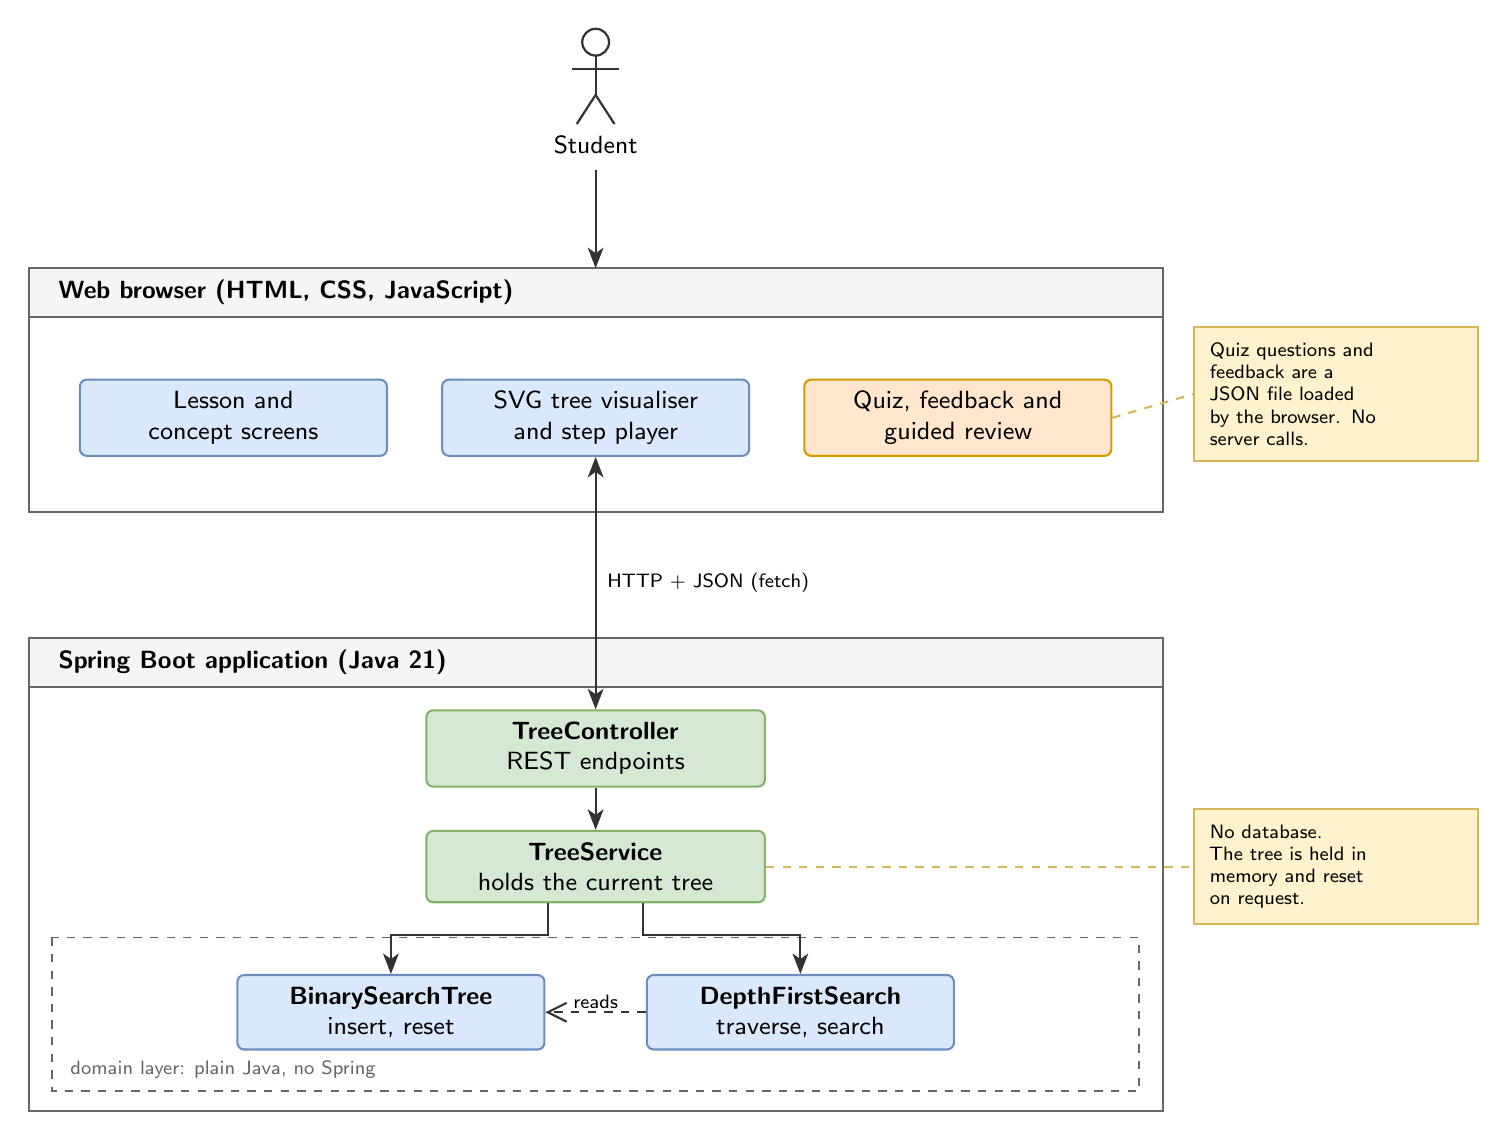
\begin{tikzpicture}[dio]
  \actor{0}{1.75}{Student}{stu}
  % Browser lane
  \lane{-7.2}{-0.5}{7.2}{-3.6}{Web browser (HTML, CSS, JavaScript)}{dioGrey}
  \node[box, text width=36mm] (lesson) at (-4.6,-2.4) {Lesson and\\ concept screens};
  \node[box, text width=36mm] (viz)    at (0,-2.4)    {SVG tree visualiser\\ and step player};
  \node[boxc={dioOrange}{text width=36mm}] (quiz) at (4.6,-2.4) {Quiz, feedback and\\ guided review};
  % Server lane
  \lane{-7.2}{-5.2}{7.2}{-11.2}{Spring Boot application (Java 21)}{dioGrey}
  \node[boxc={dioGreen}{text width=40mm}] (ctrl) at (0,-6.6) {\textbf{TreeController}\\ REST endpoints};
  \node[boxc={dioGreen}{text width=40mm}] (svc)  at (0,-8.1) {\textbf{TreeService}\\ holds the current tree};
  \node[box, text width=36mm] (bst) at (-2.6,-9.95) {\textbf{BinarySearchTree}\\ insert, reset};
  \node[box, text width=36mm] (dfs) at (2.6,-9.95)  {\textbf{DepthFirstSearch}\\ traverse, search};
  \node[font=\sffamily\scriptsize, text=dioGreyLine, anchor=south west] at (-6.8,-10.92)
       {domain layer: plain Java, no Spring};
  \draw[draw=dioGreyLine, dashed, line width=0.6pt] (-6.9,-9.0) rectangle (6.9,-10.95);
  % notes
  \node[note, text width=32mm] (n1) at (9.4,-2.1) {Quiz questions and\\ feedback are a\\ JSON file loaded\\ by the browser. No\\ server calls.};
  \node[note, text width=32mm] (n2) at (9.4,-8.1) {No database.\\ The tree is held in\\ memory and reset\\ on request.};
  % edges
  \draw[arrow] (0,0.75) -- (0,-0.5);
  \draw[arrow, <->] (viz.south) -- node[lbl, right=1mm] {HTTP + JSON (fetch)} (ctrl.north);
  \draw[arrow] (ctrl) -- (svc);
  \draw[arrow] (svc.south) ++(-0.6,0) |- ++(0,-0.4) -| (bst.north);
  \draw[arrow] (svc.south) ++(0.6,0) |- ++(0,-0.4) -| (dfs.north);
  \draw[dep] (dfs.west) -- node[lbl, above] {reads} (bst.east);
  \draw[draw=dioYellowLine, dashed] (quiz.east) -- (n1.west);
  \draw[draw=dioYellowLine, dashed] (svc.east) -- (n2.west);
\end{tikzpicture}}
\caption{Layered architecture of the COS212 DFS Tutor.}
\label{fig:arch}
\end{figure}

\textbf{How a request flows}
\begin{enumerate}
  \item The student opens \code{http://localhost:8080} and the browser loads the static files.
  \item The student chooses an action, for example ``Search for 60''.
  \item JavaScript checks the input, then sends a request to the Spring Boot backend.
  \item The controller passes the request to the service.
  \item The service asks \code{DepthFirstSearch} to run over the current \code{BinarySearchTree}.
  \item The algorithm records every step (visited node, stack contents, explanation) and returns them.
  \item The backend sends the result back as JSON.
  \item The browser plays the steps back one at a time as the student clicks ``Next''.
\end{enumerate}

Returning all the steps in one response, rather than calling the server once per step, keeps the
step player fast and lets the student go backwards as well as forwards.

% =====================================================================
\section{UML models}
% =====================================================================

\subsection{Use case diagram}

The only actor is the student. There is no lecturer or administrator role in the prototype.

\begin{figure}[H]
\centering
\resizebox{0.95\linewidth}{!}{%
\begin{tikzpicture}[dio]
  \draw[draw=dioGreyLine, fill=white, line width=0.75pt] (2.6,0.2) rectangle (13.6,-12.0);
  \node[font=\sffamily\small\bfseries, anchor=north] at (8.1,0.05) {COS212 DFS Tutor};
  \actor{0}{-6.0}{Student}{st}
  \node[usecase] (u1) at (5.3,-1.3)  {Work through\\ DFS lesson};
  \node[usecase] (u2) at (5.3,-2.9)  {View example tree};
  \node[usecase] (u3) at (5.3,-4.5)  {Insert a value};
  \node[usecase] (u4) at (5.3,-6.1)  {Run DFS traversal\\ (pre / in / post)};
  \node[usecase] (u5) at (5.3,-7.7)  {Search with DFS};
  \node[usecase] (u6) at (5.3,-9.3)  {Take readiness quiz};
  \node[usecase] (u7) at (5.3,-10.9) {Reset tree};
  \node[usecase] (s1) at (11.0,-6.9) {Step through visits\\ and stack};
  \node[usecase] (s2) at (11.0,-4.3) {Predict the next node};
  \node[usecase] (s3) at (11.0,-9.3) {Receive feedback};
  \node[usecase] (s4) at (11.0,-11.0) {Get guided review};
  \foreach \u in {u1,u2,u3,u4,u5,u6,u7} \draw[draw=edge, line width=0.75pt] (st) -- (\u.west);
  \draw[dep] (u4.east) -- node[lbl, above, sloped] {\guillemotleft include\guillemotright} (s1.west);
  \draw[dep] (u5.east) -- node[lbl, below, sloped] {\guillemotleft include\guillemotright} (s1.west);
  \draw[dep] (s2.south) -- node[lbl, right] {\guillemotleft extend\guillemotright} (s1.north);
  \draw[dep] (u6.east) -- node[lbl, above] {\guillemotleft include\guillemotright} (s3.west);
  \draw[dep] (s4.north west) -- node[lbl, below, sloped, pos=0.55] {\guillemotleft extend\guillemotright} (u6.south east);
  \node[note, anchor=west] at (8.6,-1.4) {extend condition for guided review:\\ quiz score below 4/6};
\end{tikzpicture}}
\caption{Use case diagram.}
\label{fig:usecase}
\end{figure}

\subsection{Sequence diagram: DFS search for a value}

This shows what happens between the browser and the backend classes when a student searches for 60.

\begin{figure}[H]
\centering
\resizebox{\linewidth}{!}{%
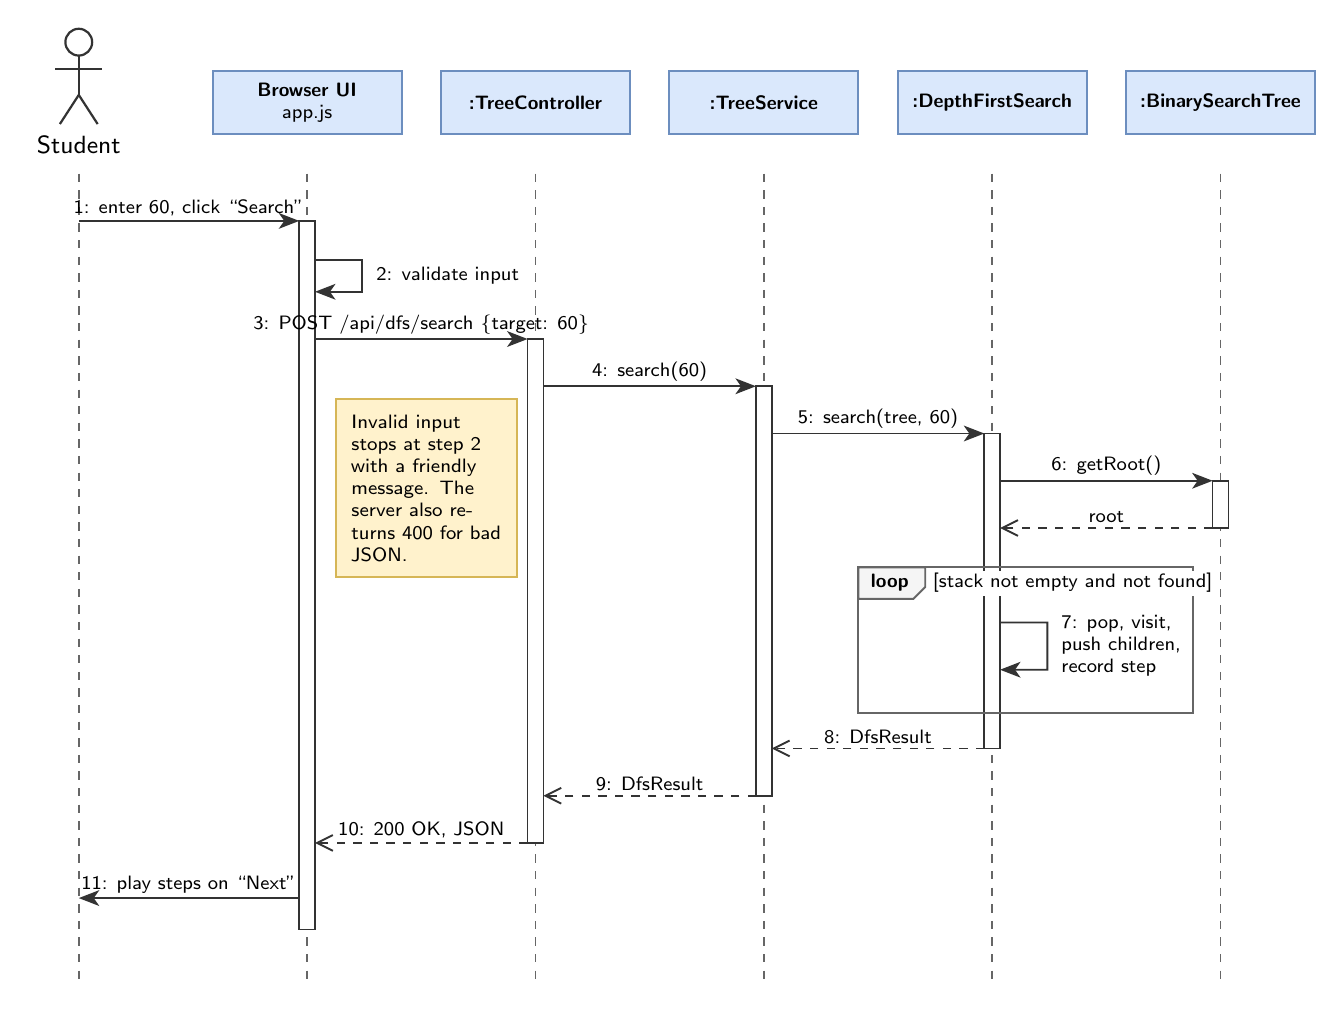
\begin{tikzpicture}[dio, font=\sffamily\scriptsize]
  \tikzset{ll/.style={draw=dioBlueLine, fill=dioBlueFill, minimum width=24mm, minimum height=8mm,
                      font=\sffamily\scriptsize\bfseries, align=center},
           act/.style={draw=edge, fill=white, line width=0.6pt},
           msg/.style={->, draw=edge, line width=0.7pt},
           mlbl/.style={font=\sffamily\scriptsize, above, inner sep=1.5pt}}
  % lifeline heads
  \actor{0}{0.15}{Student}{s}
  \node[ll] (ui)  at (2.9,0)  {Browser UI\\ \textmd{app.js}};
  \node[ll] (tc)  at (5.8,0)  {:TreeController};
  \node[ll] (ts)  at (8.7,0)  {:TreeService};
  \node[ll] (df)  at (11.6,0) {:DepthFirstSearch};
  \node[ll] (bt)  at (14.5,0) {:BinarySearchTree};
  \foreach \x in {0,2.9,5.8,8.7,11.6,14.5}
    \draw[draw=dioGreyLine, dashed, line width=0.6pt] (\x,-0.9) -- (\x,-11.2);
  % activation bars
  \filldraw[act] (2.8,-1.5) rectangle (3.0,-10.5);
  \filldraw[act] (5.7,-3.0) rectangle (5.9,-9.4);
  \filldraw[act] (8.6,-3.6) rectangle (8.8,-8.8);
  \filldraw[act] (11.5,-4.2) rectangle (11.7,-8.2);
  \filldraw[act] (14.4,-4.8) rectangle (14.6,-5.4);
  % messages
  \draw[msg] (0,-1.5) -- node[mlbl] {1: enter 60, click ``Search''} (2.8,-1.5);
  \draw[msg] (3.0,-2.0) -- ++(0.6,0) -- ++(0,-0.4) -- node[mlbl, right, pos=0] {} (3.0,-2.4);
  \node[font=\sffamily\scriptsize, anchor=west] at (3.65,-2.2) {2: validate input};
  \draw[msg] (3.0,-3.0) -- node[mlbl] {3: POST /api/dfs/search \{target: 60\}} (5.7,-3.0);
  \draw[msg] (5.9,-3.6) -- node[mlbl] {4: search(60)} (8.6,-3.6);
  \draw[msg] (8.8,-4.2) -- node[mlbl] {5: search(tree, 60)} (11.5,-4.2);
  \draw[msg] (11.7,-4.8) -- node[mlbl] {6: getRoot()} (14.4,-4.8);
  \draw[ret] (14.4,-5.4) -- node[mlbl] {root} (11.7,-5.4);
  % loop fragment
  \draw[draw=dioGreyLine, line width=0.7pt] (9.9,-5.9) rectangle (14.15,-7.75);
  \draw[draw=dioGreyLine, fill=dioGreyFill, line width=0.7pt]
       (9.9,-5.9) -- (10.75,-5.9) -- (10.75,-6.15) -- (10.6,-6.3) -- (9.9,-6.3) -- cycle;
  \node[font=\sffamily\scriptsize\bfseries] at (10.3,-6.1) {loop};
  \node[font=\sffamily\scriptsize, anchor=west, fill=white, inner sep=1pt] at (10.8,-6.1) {[stack not empty and not found]};
  \draw[msg] (11.7,-6.6) -- ++(0.6,0) -- ++(0,-0.6) -- (11.7,-7.2);
  \node[font=\sffamily\scriptsize, anchor=west, align=left] at (12.35,-6.9) {7: pop, visit,\\ push children,\\ record step};
  % returns
  \draw[ret] (11.5,-8.2) -- node[mlbl] {8: DfsResult} (8.8,-8.2);
  \draw[ret] (8.6,-8.8) -- node[mlbl] {9: DfsResult} (5.9,-8.8);
  \draw[ret] (5.7,-9.4) -- node[mlbl] {10: 200 OK, JSON} (3.0,-9.4);
  \draw[msg] (2.8,-10.1) -- node[mlbl] {11: play steps on ``Next''} (0,-10.1);
  % note
  \node[note, text width=19mm, anchor=north west] at (3.25,-3.75)
       {Invalid input stops at step 2 with a friendly message. The server also returns 400 for
        bad JSON.};
\end{tikzpicture}}
\caption{Sequence diagram for a DFS search.}
\label{fig:sequence}
\end{figure}

\subsection{Activity diagram: the DFS search algorithm}

\begin{figure}[H]
\centering
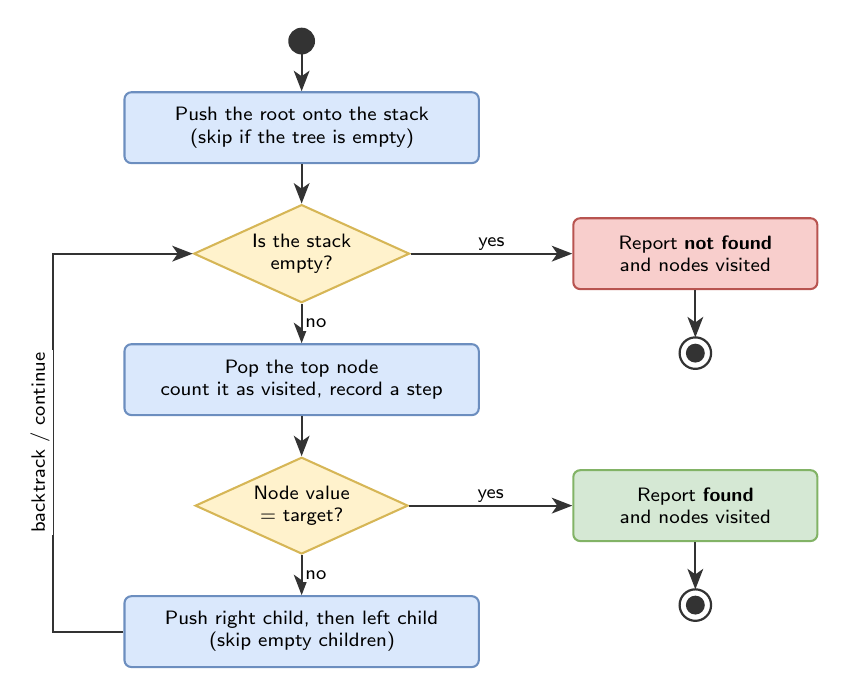
\begin{tikzpicture}[dio, font=\sffamily\scriptsize]
  \tikzset{actn/.style={box, minimum width=44mm, text width=42mm, font=\sffamily\scriptsize},
           dec/.style={diamond, aspect=2.2, draw=dioYellowLine, fill=dioYellowFill, align=center,
                       inner sep=0.6mm, font=\sffamily\scriptsize},
           endn/.style={boxc={dioGreen}{minimum width=30mm, text width=28mm, font=\sffamily\scriptsize}},
           endr/.style={boxc={dioRed}{minimum width=30mm, text width=28mm, font=\sffamily\scriptsize}}}
  \fill[edge] (0,0) circle (0.17);
  \node[actn] (a1) at (0,-1.1) {Push the root onto the stack\\ (skip if the tree is empty)};
  \node[dec]  (d1) at (0,-2.7) {Is the stack\\ empty?};
  \node[actn] (a2) at (0,-4.3) {Pop the top node\\ count it as visited, record a step};
  \node[dec]  (d2) at (0,-5.9) {Node value\\ = target?};
  \node[actn] (a3) at (0,-7.5) {Push right child, then left child\\ (skip empty children)};
  \node[endr] (nf) at (5.0,-2.7) {Report \textbf{not found}\\ and nodes visited};
  \node[endn] (fd) at (5.0,-5.9) {Report \textbf{found}\\ and nodes visited};
  \draw[arrow] (0,-0.17) -- (a1);
  \draw[arrow] (a1) -- (d1);
  \draw[arrow] (d1) -- node[lbl, right] {no} (a2);
  \draw[arrow] (a2) -- (d2);
  \draw[arrow] (d2) -- node[lbl, right] {no} (a3);
  \draw[arrow] (d1) -- node[lbl, above] {yes} (nf);
  \draw[arrow] (d2) -- node[lbl, above] {yes} (fd);
  \draw[arrow] (a3.west) -- ++(-0.9,0) |- (d1.west);
  \node[lbl, rotate=90, anchor=south] at (-3.15,-5.1) {backtrack / continue};
  % final nodes
  \foreach \n in {nf, fd} {
    \draw[arrow] (\n.south) -- ++(0,-0.6);
    \draw[edge, line width=0.8pt] ($(\n.south)+(0,-0.8)$) circle (0.2);
    \fill[edge] ($(\n.south)+(0,-0.8)$) circle (0.12);
  }
\end{tikzpicture}
\caption{Activity diagram for the iterative DFS search used in the app.}
\label{fig:activity}
\end{figure}

\subsection{Class diagram}

\begin{figure}[H]
\centering
\resizebox{\linewidth}{!}{%
\begin{tikzpicture}[dio]
  \node[umlclass, anchor=north] (ctrl) at (0,0) {%
    \textbf{TreeController}
    \nodepart{two} -- service : TreeService
    \nodepart{three} + getTree() : TreeView\\
                     + insert(req : InsertRequest) : TreeView\\
                     + search(req : SearchRequest) : DfsResult\\
                     + traverse(req : TraverseRequest) : DfsResult\\
                     + reset() : TreeView};
  \node[umlclass, anchor=north] (svc) at (6.3,0) {%
    \textbf{TreeService}
    \nodepart{two} -- tree : BinarySearchTree\\ -- dfs : DepthFirstSearch
    \nodepart{three} + getTree() : TreeView\\
                     + insert(value : int) : TreeView\\
                     + search(target : int) : DfsResult\\
                     + traverse(order : TraversalOrder) : DfsResult\\
                     + reset() : TreeView};
  \node[umlclass, anchor=north] (bst) at (12.6,0) {%
    \textbf{BinarySearchTree}
    \nodepart{two} -- root : TreeNode\\ -- size : int
    \nodepart{three} + insert(value : int) : boolean\\
                     + getRoot() : TreeNode\\
                     + size() : int\\
                     + clear() : void};
  \node[umlclass, anchor=north] (dfs) at (6.3,-4.6) {%
    \textbf{DepthFirstSearch}
    \nodepart{two} \textit{(no state)}
    \nodepart{three} + search(tree, target : int) : DfsResult\\
                     + traverse(tree, order) : DfsResult};
  \node[umlclass, anchor=north] (node) at (12.6,-4.6) {%
    \textbf{TreeNode}
    \nodepart{two} -- value : int\\ -- left : TreeNode\\ -- right : TreeNode
    \nodepart{three} + getValue() : int\\ + getLeft() : TreeNode\\ + getRight() : TreeNode};
  \node[umlclass, anchor=north] (res) at (6.3,-8.2) {%
    \textbf{DfsResult}
    \nodepart{two} -- order : TraversalOrder\\ -- target : Integer\\ -- found : boolean\\
                   -- visitOrder : List\textless Integer\textgreater\\ -- steps : List\textless DfsStep\textgreater
    \nodepart{three} + nodesVisited() : int};
  \node[umlclass, anchor=north] (step) at (12.6,-8.2) {%
    \textbf{DfsStep}
    \nodepart{two} -- number : int\\ -- node : int\\ -- stackAfter : List\textless Integer\textgreater\\
                   -- explanation : String
    \nodepart{three} \textit{(record: accessors only)}};
  \node[umlenum, anchor=north] (ord) at (0,-8.2) {%
    \textit{\guillemotleft enumeration\guillemotright}\\ \textbf{TraversalOrder}
    \nodepart{two} PRE\_ORDER\\ IN\_ORDER\\ POST\_ORDER};
  \node[note, text width=40mm, anchor=north] at (0,-4.6)
    {BinarySearchTree, TreeNode, DepthFirstSearch, DfsResult and DfsStep live in the
     \texttt{model} package and have no Spring imports, so JUnit tests them directly.};
  % relationships
  \draw[arrow] (ctrl.east |- 0,-1.0) -- node[lbl, above] {1} (svc.west |- 0,-1.0);
  % composition: service owns tree
  \draw[draw=edge, line width=0.75pt, {Diamond[length=3mm,width=2mm,fill=edge]}->] (svc.east |- 0,-1.0) -- node[lbl, above, pos=0.8] {1} (bst.west |- 0,-1.0);
  \draw[arrow] (svc.south) -- node[lbl, right] {1} (dfs.north);
  \draw[draw=edge, line width=0.75pt, {Diamond[length=3mm,width=2mm,fill=edge]}->] (bst.south) -- node[lbl, right] {root 0..1} (node.north);
  % self association
  \draw[arrow] (node.east |- 0,-5.6) -- ++(0.6,0) |- node[lbl, right, pos=0.25] {left, right 0..2} (node.east |- 0,-6.6);
  \draw[dep] (dfs.east |- 0,-5.4) -- node[lbl, above] {\guillemotleft reads\guillemotright} (node.west |- 0,-5.4);
  \draw[dep] (dfs.south) -- node[lbl, right] {\guillemotleft creates\guillemotright} (res.north);
  \draw[draw=edge, line width=0.75pt, {Diamond[length=3mm,width=2mm,fill=edge]}->] (res.east |- 0,-9.0) -- node[lbl, above, pos=0.75] {0..*} (step.west |- 0,-9.0);
  \draw[arrow] (res.west |- 0,-9.0) -- node[lbl, above] {1} (ord.east |- 0,-9.0);
\end{tikzpicture}}
\caption{Class diagram for the Java backend (DTOs such as \code{TreeView} and the request records are omitted for clarity).}
\label{fig:class}
\end{figure}

\textbf{Responsibilities}
\begin{itemize}
  \item \code{TreeNode}: stores a value and references to its left and right children.
  \item \code{BinarySearchTree}: builds the tree by the BST rule; rejects duplicates; can be cleared.
  \item \code{DepthFirstSearch}: runs DFS (search or traversal) over a tree and records every step.
        It never changes the tree.
  \item \code{DfsResult} and \code{DfsStep}: immutable records holding the outcome, the visit order and the
        step-by-step history used by the step player.
  \item \code{TraversalOrder}: the three depth-first orders.
  \item \code{TreeService}: owns the current tree, seeds the example tree, enforces the 15-node limit.
  \item \code{TreeController}: exposes the HTTP endpoints and turns errors into friendly 400 responses.
  \item \code{TreeView} (DTO): a nested JSON-friendly copy of the tree for the visualiser.
\end{itemize}

\subsection{Deployment diagram}

\begin{figure}[H]
\centering
\resizebox{0.9\linewidth}{!}{%
\begin{tikzpicture}[dio]
  \depnode{0}{0}{6.2}{-4.6}{\guillemotleft device\guillemotright\\ \textbf{Student laptop}}{dioGrey}
  \draw[draw=dioBlueLine, fill=white, line width=0.7pt] (0.4,-1.3) rectangle (5.8,-4.2);
  \node[font=\sffamily\scriptsize, align=center] at (3.1,-1.65) {\guillemotleft execution environment\guillemotright\ \textbf{Web browser}};
  \node[boxc={dioBlue}{minimum width=44mm, text width=42mm, font=\sffamily\scriptsize}] at (3.1,-3.1)
       {\guillemotleft artifact\guillemotright\\ index.html, app.js, styles.css\\ quiz-bank.json};
  \depnode{9.0}{0}{15.6}{-4.6}{\guillemotleft device\guillemotright\\ \textbf{Host machine}}{dioGrey}
  \draw[draw=dioGreenLine, fill=white, line width=0.7pt] (9.4,-1.3) rectangle (15.2,-4.2);
  \node[font=\sffamily\scriptsize, align=center] at (12.3,-1.65) {\guillemotleft execution environment\guillemotright\ \textbf{JVM (Java 21)}};
  \node[boxc={dioGreen}{minimum width=44mm, text width=42mm, font=\sffamily\scriptsize}] at (12.3,-3.1)
       {\guillemotleft artifact\guillemotright\\ dfs-tutor.jar\\ (Spring Boot, embedded Tomcat,\\ in-memory tree)};
  \draw[draw=edge, line width=0.8pt] (6.2,-2.6) -- node[lbl, above] {\guillemotleft HTTP\guillemotright} node[lbl, below] {port 8080} (9.0,-2.6);
  \node[note, text width=80mm, anchor=north] at (7.8,-5.3)
       {For development and the examination demo both nodes are the same laptop
        (\texttt{localhost:8080}). The JAR can later be moved to any machine with Java 21.};
\end{tikzpicture}}
\caption{Deployment diagram.}
\label{fig:deploy}
\end{figure}

% =====================================================================
\section{Backend API}
% =====================================================================

\begin{tabularx}{\textwidth}{@{}l l L@{}}
  \toprule
  \textbf{Method} & \textbf{Endpoint} & \textbf{Purpose} \\
  \midrule
  \code{GET}  & \code{/api/tree}          & Return the current tree. \\
  \code{POST} & \code{/api/tree/insert}   & Insert an integer: \code{\{"value": 65\}}. \\
  \code{POST} & \code{/api/tree/reset}    & Restore the example tree. \\
  \code{POST} & \code{/api/dfs/search}    & DFS search: \code{\{"target": 60\}}. \\
  \code{POST} & \code{/api/dfs/traverse}  & DFS traversal: \code{\{"order": "IN\_ORDER"\}}. \\
  \bottomrule
\end{tabularx}

\subsection{Successful search}

\code{POST /api/dfs/search} with body \code{\{"target": 60\}} returns:

\begin{lstlisting}[style=json]
{
  "order": "PRE_ORDER",
  "target": 60,
  "found": true,
  "visitOrder": [50, 30, 20, 40, 70, 60],
  "nodesVisited": 6,
  "steps": [
    { "number": 1, "node": 50, "stackAfter": [30, 70],
      "explanation": "Visit 50. It is not 60. Push 70 (right), then 30 (left), so 30 is on top." },
    { "number": 2, "node": 30, "stackAfter": [20, 40, 70],
      "explanation": "Visit 30. Not 60. Push 40, then 20." },
    ...
    { "number": 6, "node": 60, "stackAfter": [80],
      "explanation": "Visit 60. This is the target. Stop searching." }
  ]
}
\end{lstlisting}

\code{stackAfter} lists the stack top first. The browser uses \code{steps} to drive the step
player and the stack panel, so it never has to work out the algorithm itself (NFR-03).

\subsection{Unsuccessful search}

\begin{lstlisting}[style=json]
{
  "order": "PRE_ORDER",
  "target": 65,
  "found": false,
  "visitOrder": [50, 30, 20, 40, 70, 60, 80],
  "nodesVisited": 7,
  "steps": [ ... ]
}
\end{lstlisting}

\subsection{Traversal}

\code{POST /api/dfs/traverse} with \code{\{"order": "IN\_ORDER"\}} returns the same shape with
\code{target} set to \code{null}, \code{found} set to \code{false} and
\code{"visitOrder": [20, 30, 40, 50, 60, 70, 80]}. For traversals \code{stackAfter} holds the
recursion (call) stack, which is the path from the root to the current node.

\subsection{Error handling}

All errors use HTTP \code{400 Bad Request} (or \code{500} for unexpected faults) and a body the
frontend can show directly:

\begin{lstlisting}[style=json]
{ "error": "DUPLICATE_VALUE",
  "message": "40 is already in the tree. Each value can appear only once in this BST." }
\end{lstlisting}

\begin{tabularx}{\textwidth}{@{}l L@{}}
  \toprule
  \textbf{Error code} & \textbf{When} \\
  \midrule
  \code{MISSING\_VALUE}  & Target or value is missing. \\
  \code{INVALID\_NUMBER} & Not a whole number, or outside 0--99. \\
  \code{INVALID\_ORDER}  & Order is not one of the three allowed values. \\
  \code{DUPLICATE\_VALUE} & Inserting a value that already exists. \\
  \code{TREE\_FULL}      & Inserting a sixteenth node. \\
  \code{INTERNAL\_ERROR} & Anything unexpected. The message is generic; details go to the server log. \\
  \bottomrule
\end{tabularx}

% =====================================================================
\section{Core algorithm}
% =====================================================================

The search is written iteratively with an explicit stack, because the stack is exactly what we
want students to see. The traversal is written recursively, because it shows very compactly that
the three orders differ only in where one line sits.

\begin{lstlisting}[style=java, caption={DFS search (iterative, pre-order).}]
public DfsResult search(BinarySearchTree tree, int target) {
    DfsResult.Builder result = DfsResult.builder(TraversalOrder.PRE_ORDER, target);
    Deque<TreeNode> stack = new ArrayDeque<>();
    if (tree.getRoot() != null) {
        stack.push(tree.getRoot());
    }
    while (!stack.isEmpty()) {
        TreeNode current = stack.pop();
        if (current.getValue() == target) {
            result.visit(current.getValue(), stack, "This is the target. Stop searching.");
            return result.found();
        }
        // Push right first so that left ends up on top and is explored first.
        if (current.getRight() != null) stack.push(current.getRight());
        if (current.getLeft() != null)  stack.push(current.getLeft());
        result.visit(current.getValue(), stack, explain(current));
    }
    return result.notFound();
}
\end{lstlisting}

\begin{lstlisting}[style=java, caption={DFS traversal (recursive). Only the position of \texttt{visit} changes between orders.}]
private void walk(TreeNode node, TraversalOrder order,
                  Deque<Integer> path, DfsResult.Builder result) {
    if (node == null) return;
    path.push(node.getValue());
    if (order == TraversalOrder.PRE_ORDER)  result.visit(node.getValue(), path);
    walk(node.getLeft(), order, path, result);
    if (order == TraversalOrder.IN_ORDER)   result.visit(node.getValue(), path);
    walk(node.getRight(), order, path, result);
    if (order == TraversalOrder.POST_ORDER) result.visit(node.getValue(), path);
    path.pop();
}
\end{lstlisting}

Both run in $O(n)$ time for a tree of $n$ nodes, since each node is visited at most once. The extra
space is $O(h)$, where $h$ is the height of the tree: about $\log_2 n$ for a balanced tree and up
to $n$ for a skewed one. FR-15 lets students see this difference.

% =====================================================================
\section{Project structure}
% =====================================================================

\begin{lstlisting}[basicstyle=\ttfamily\footnotesize, backgroundcolor=\color{codebg}, frame=single, rulecolor=\color{black!15}]
cos212-dfs-tutor/
|-- pom.xml
|-- README.md
|-- docs/
|   |-- SE-document.tex          (this document)
|   `-- ID-document.tex
`-- src/
    |-- main/
    |   |-- java/za/ac/up/dfstutor/
    |   |   |-- DfsTutorApplication.java
    |   |   |-- controller/  TreeController.java, ApiExceptionHandler.java
    |   |   |-- service/     TreeService.java
    |   |   |-- model/       TreeNode.java, BinarySearchTree.java,
    |   |   |                DepthFirstSearch.java, TraversalOrder.java,
    |   |   |                DfsResult.java, DfsStep.java
    |   |   `-- dto/         InsertRequest.java, SearchRequest.java,
    |   |                    TraverseRequest.java, TreeView.java, ApiError.java
    |   `-- resources/
    |       |-- application.properties
    |       `-- static/
    |           |-- index.html
    |           |-- css/styles.css
    |           |-- js/app.js, js/tree-view.js, js/step-player.js, js/quiz.js
    |           `-- data/quiz-bank.json, data/lesson.json
    `-- test/java/za/ac/up/dfstutor/
        |-- BinarySearchTreeTest.java
        |-- DepthFirstSearchTest.java
        `-- TreeControllerTest.java
\end{lstlisting}

This is enough for the first version. We avoid extra interfaces, factories and repositories unless
the code gives us a concrete reason to add them. Lesson text and quiz questions live in JSON files
so that the ID team can edit content without touching JavaScript.

% =====================================================================
\section{Testing and acceptance}
% =====================================================================

\subsection{Unit tests (JUnit 5)}

\begin{itemize}
  \item Empty tree: search returns not found with 0 nodes visited.
  \item Root as target: found after 1 visit.
  \item Search for 60 on the example tree: visit order is exactly 50, 30, 20, 40, 70, 60.
  \item Search for 65: not found, all 7 nodes visited.
  \item Pre-, in- and post-order on the example tree match Table~\ref{tab:orders}.
  \item In-order of any tree built from random distinct values is sorted (property-style test).
  \item \code{stackAfter} for every step of the 60 search matches Table~\ref{tab:trace}.
  \item Skewed tree (10, 20, 30, 40): every order is correct and the stack never holds more than one
        pending right child.
  \item Inserting a duplicate returns \code{false} and leaves the tree unchanged.
  \item Inserting a sixteenth value is rejected by the service.
\end{itemize}

\subsection{Acceptance criteria}

The prototype is ready to demonstrate when every check below passes.

\begin{longtable}{@{}p{5.6cm} p{9.4cm}@{}}
  \toprule
  \textbf{Check} & \textbf{Expected result} \\
  \midrule
  \endhead
  Open the app & The introduction is shown, followed by the example tree. \\
  Pre-order traversal & Visits 50, 30, 20, 40, 70, 60, 80 with the stack shown at each step. \\
  In-order traversal & Visits 20 to 80 in sorted order; the app points out that it is sorted. \\
  Post-order traversal & Visits 20, 40, 30, 60, 80, 70, 50. \\
  Search for the root (50) & Found after 1 visit. \\
  Search for 60 & Found after 6 visits; the whole left subtree is explored first. \\
  Search for a missing value (65) & ``Not found'' after visiting all 7 nodes. \\
  Step backwards & The previous step, highlight and stack are restored exactly. \\
  Predict the next node, correctly & Confirmation with a one-line reason. \\
  Predict the next node, incorrectly & Explanation of the mistake and a hint; the student can try again. \\
  Insert a valid integer & The node appears in the correct position. \\
  Insert a duplicate & Message explaining that the value already exists. \\
  Insert invalid input (``abc'', 150) & Friendly validation message; nothing is sent to the server for ``abc''. \\
  Reset the tree & The example tree is restored. \\
  Quiz score 4/6 or higher & Summary screen with questions for the lecture. \\
  Quiz score below 4/6 & Guided review is offered for the missed outcomes, then a new quiz variant. \\
  Keyboard only & Every screen can be completed without a mouse. \\
  \bottomrule
\end{longtable}

\subsection{Peer evaluation}

Between days 11 and 12, at least three students who have not taken COS212 yet (or who have
forgotten DFS) use the app without help while a group member observes. We note where they hesitate,
what they misread and how long a session takes. Changes are limited to fixes that remove confusion;
new features are not added at this stage. A short summary of findings goes into the ID document's
evaluation section.

% =====================================================================
\section{Development plan}
\label{sec:plan}
% =====================================================================

Today is Wednesday 28 October 2026. Documentation is due on ClickUP before 08:00 on Monday
16 November, and the presentation is on 16 or 17 November. The plan below finishes the prototype
by 11 November and leaves four days of buffer.

\begin{longtable}{@{}p{1.2cm} p{2.8cm} p{6.6cm} p{4.4cm}@{}}
  \toprule
  \textbf{Days} & \textbf{Dates} & \textbf{Work} & \textbf{Done when\ldots} \\
  \midrule
  \endhead
  1--2   & 29--30 Oct  & Approve this document; create repository; Spring Boot skeleton; start ID document outline. & App starts and shows a placeholder page. \\
  3--4   & 31 Oct--1 Nov & \code{BinarySearchTree}, \code{DepthFirstSearch}, step recording, JUnit tests. & All unit tests pass. \\
  5--6   & 2--3 Nov    & REST endpoints and error handling; first end-to-end search from the browser. & Search works through HTTP. \\
  7--8   & 4--5 Nov    & SVG tree, step player, stack panel, highlights. & Students can watch DFS work. \\
  9--10  & 6--7 Nov    & Lesson screens, predict mode, quiz, feedback, guided review. & Full learning journey works. \\
  11--12 & 8--9 Nov    & Edge cases, accessibility pass, peer testing, bug fixes. & Acceptance checks pass. \\
  13     & 10 Nov      & Finalise SE and ID documents, README, slides. & Documents ready to submit. \\
  14     & 11 Nov      & Full rehearsal (10 min talk + 10 min demo); tag release \code{v1.0}. & Demo runs cleanly twice. \\
  ---    & 12--15 Nov  & Buffer. Submit documents early. & --- \\
  \bottomrule
\end{longtable}

\textbf{One rule we will stick to:} integrate as soon as the first search endpoint works (day 5 or 6).
We do not wait for the frontend to be finished before testing it against the real Java backend.

\textbf{Other deadlines.} Self-reflection reports are individual and due before 20:00 on
Wednesday 18 November 2026.

% =====================================================================
\section{Risks}
% =====================================================================

\begin{tabularx}{\textwidth}{@{}L l L@{}}
  \toprule
  \textbf{Risk} & \textbf{Likelihood} & \textbf{What we do about it} \\
  \midrule
  The step player takes longer than planned. & Medium & Build a plain list view of the steps first; add animation only if time allows. \\
  Frontend and backend disagree on the JSON. & Medium & Agree the JSON examples in this document on day 2 and integrate early. \\
  Skewed trees do not fit on screen. & Low & 15-node limit; SVG scales to fit and scrolls vertically. \\
  Quiz content is wrong or confusing. & Medium & Every item is checked against the Java output by two members. \\
  The demo fails on the day (laptop, projector). & Low & Run locally with no internet; keep a built JAR on two laptops and a short screen recording as backup. \\
  A member becomes unavailable. & Medium & Pair on every component so at least two people know each part. \\
  \bottomrule
\end{tabularx}

% =====================================================================
\section{Decisions for the team to approve}
% =====================================================================

Before development starts, every member should agree to the following:

\begin{enumerate}
  \item Data structure: binary search tree. Algorithm: depth-first search (search and the three traversal orders).
  \item Java 21 with Spring Boot 3 (or Java 17 if that is what members already have), built with Maven.
  \item Plain HTML, CSS and JavaScript served by Spring Boot; no frontend framework.
  \item No database and no user accounts in the first version.
  \item Values 0--99, at most 15 nodes, duplicates rejected.
  \item The backend returns every DFS step; the browser only displays them.
  \item Gagné's Nine Events structures the lesson; ADDIE structures the project.
  \item Quiz pass threshold of 4/6, with guided review below that.
  \item GitHub Issues and pull requests for all work; every pull request is reviewed by one other member.
\end{enumerate}

Once these are approved, the next step is to create the GitHub repository, initialise the Spring
Boot project and assign the first two tasks: the BST and DFS implementation with tests, and the
basic frontend shell.

% =====================================================================
\begin{thebibliography}{99}
\bibitem{cs2023} A.\,N. Kumar, R.\,K. Raj, S.\,G. Aly, M.\,D. Anderson, B.\,A. Becker et al.
  \emph{Computer Science Curricula 2023}. Association for Computing Machinery, New York, 2024.
\bibitem{anderson2001} L.\,W. Anderson and D.\,R. Krathwohl (eds.). \emph{A Taxonomy for Learning,
  Teaching, and Assessing: A Revision of Bloom's Taxonomy of Educational Objectives}. Longman, 2001.
\bibitem{gagne2005} R.\,M. Gagn\'e, W.\,W. Wager, K.\,C. Golas and J.\,M. Keller.
  \emph{Principles of Instructional Design}, 5th ed. Wadsworth, 2005.
\bibitem{sweller1988} J. Sweller. Cognitive load during problem solving: effects on learning.
  \emph{Cognitive Science}, 12(2):257--285, 1988.
\bibitem{hundhausen2002} C.\,D. Hundhausen, S.\,A. Douglas and J.\,T. Stasko. A meta-study of
  algorithm visualization effectiveness. \emph{Journal of Visual Languages and Computing},
  13(3):259--290, 2002.
\bibitem{naps2002} T.\,L. Naps, G. R\"o{\ss}ling et al. Exploring the role of visualization and
  engagement in computer science education. \emph{ACM SIGCSE Bulletin}, 35(2):131--152, 2003
  (ITiCSE 2002 working group report).
\bibitem{vygotsky1978} L.\,S. Vygotsky. \emph{Mind in Society: The Development of Higher
  Psychological Processes}. Harvard University Press, 1978.
\bibitem{mayer2009} R.\,E. Mayer. \emph{Multimedia Learning}, 2nd ed. Cambridge University Press, 2009.
\bibitem{pashler2008} H. Pashler, M. McDaniel, D. Rohrer and R. Bjork. Learning styles: concepts
  and evidence. \emph{Psychological Science in the Public Interest}, 9(3):105--119, 2008.
\bibitem{keller1987} J.\,M. Keller. Development and use of the ARCS model of instructional design.
  \emph{Journal of Instructional Development}, 10(3):2--10, 1987.
\end{thebibliography}

\end{document}
